% RRFA: Representation Rerouting for Agentic Safety
\documentclass[10pt, twocolumn]{article}

\usepackage[
    top=2cm, bottom=2cm, left=1.8cm, right=1.8cm,
    headheight=13pt, columnsep=0.7cm
]{geometry}

\usepackage[T1]{fontenc}
\usepackage[utf8]{inputenc}
\usepackage{lmodern}
\usepackage{microtype}
\usepackage{parskip}
\usepackage{amsmath, amssymb, amsthm}
\usepackage{mathtools}
\usepackage[dvipsnames]{xcolor}
\usepackage{booktabs}
\usepackage{array}
\usepackage{tabularx}
\usepackage{multirow}
\usepackage{colortbl}
\usepackage{tikz}
\usetikzlibrary{shapes, arrows.meta, positioning, calc, fit}
\usepackage[most]{tcolorbox}
\tcbuselibrary{skins, breakable}
\usepackage{fancyhdr}
\usepackage{lastpage}
\usepackage[colorlinks=true, linkcolor=MidnightBlue, urlcolor=MidnightBlue, citecolor=MidnightBlue]{hyperref}
\usepackage{enumitem}
\usepackage{float}
\usepackage{caption}
\usepackage{titlesec}

% --- Muted, professional color palette ---
\definecolor{seccolor}{HTML}{1a1a2e}
\definecolor{subseccolor}{HTML}{34495e}
\definecolor{rulecolor}{HTML}{bdc3c7}
\definecolor{boxframe}{HTML}{7f8c8d}
\definecolor{boxbg}{HTML}{f8f9fa}
\definecolor{defframe}{HTML}{5b6a7a}
\definecolor{resbg}{HTML}{eef7ee}
\definecolor{resframe}{HTML}{6a9a6a}
\definecolor{exbg}{HTML}{f5f5f0}
\definecolor{safe}{HTML}{2d7d46}
\definecolor{danger}{HTML}{a83232}

% --- Compact section styling ---
\titleformat{\section}{\large\bfseries\color{seccolor}}{\thesection.}{0.4em}{}[\color{rulecolor}\titlerule]
\titleformat{\subsection}{\normalsize\bfseries\color{subseccolor}}{\thesubsection}{0.4em}{}
\titleformat{\subsubsection}{\small\bfseries\color{subseccolor}}{\thesubsubsection}{0.4em}{}
\titlespacing*{\section}{0pt}{10pt}{4pt}
\titlespacing*{\subsection}{0pt}{6pt}{2pt}

% --- Header/footer ---
\pagestyle{fancy}
\fancyhf{}
\lhead{\footnotesize\color{subseccolor} RRFA: Representation Rerouting for Agentic Safety}
\rhead{\footnotesize\color{subseccolor} Internal Report -- Feb 2026}
\cfoot{\footnotesize\thepage/\pageref{LastPage}}
\renewcommand{\headrulewidth}{0.3pt}

% --- Environments ---
\newtcolorbox{defbox}[1][]{enhanced, breakable, colback=boxbg, colframe=defframe, fonttitle=\small\bfseries, title=#1, arc=1.5pt, boxrule=0.4pt, left=5pt, right=5pt, top=4pt, bottom=4pt, toptitle=2pt, bottomtitle=2pt}
\newtcolorbox{resbox}[1][]{enhanced, breakable, colback=resbg, colframe=resframe, fonttitle=\small\bfseries, title=#1, arc=1.5pt, boxrule=0.4pt, left=5pt, right=5pt, top=4pt, bottom=4pt}
\newtcolorbox{exbox}[1][]{enhanced, breakable, colback=exbg, colframe=boxframe, fonttitle=\small\bfseries, title=#1, arc=1.5pt, boxrule=0.4pt, left=5pt, right=5pt, top=3pt, bottom=3pt}

% --- Commands ---
\newcommand{\code}[1]{\texttt{\small #1}}
\newcommand{\loss}{\mathcal{L}}
\newcommand{\lrr}{\loss_{\text{rr}}}
\newcommand{\lret}{\loss_{\text{ret}}}
\newcommand{\ltotal}{\loss_{\text{total}}}
\newcommand{\hidden}{\mathbf{h}}
\newcommand{\hmodel}{\hidden_{\theta}}
\newcommand{\hfrozen}{\hidden_{\theta_0}}
\newcommand{\Ds}{D_s}
\newcommand{\Dr}{D_r}

\begin{document}

% ======================================================================
% TITLE (inline, no separate page)
% ======================================================================
\twocolumn[
\begin{@twocolumnfalse}
\begin{center}
\vspace{-0.5cm}
{\LARGE\bfseries\color{seccolor} Representation Rerouting for Agentic Safety}\\[6pt]
{\normalsize\color{subseccolor} Internal Defenses Against Prompt Injection via LoRA Circuit Breakers and Triplet Loss}\\[8pt]
{\small Internal Research Report \quad$\cdot$\quad February 2026 \quad$\cdot$\quad Base model: \texttt{Llama-3.1-8B-Instruct}}\\[4pt]
{\small\color{subseccolor} Artifacts:\; \href{https://huggingface.co/memo-ozdincer/rrfa-runs}{HF Models}\; $\cdot$\; \href{https://huggingface.co/datasets/memo-ozdincer/rrfa-data}{HF Data}}
\end{center}
\vspace{4pt}
\noindent\textcolor{rulecolor}{\rule{\textwidth}{0.5pt}}
\vspace{2pt}
\begin{quote}\small
\textbf{Abstract.}\quad
LLM agents with tool-calling capabilities are vulnerable to prompt injection attacks that hijack control flow via adversarial content in retrieved data. We present \textbf{Representation Rerouting for Agentic Safety (RRFA)}, training LoRA adapters to make harmful internal representations orthogonal to benign ones via a triplet loss with configurable loss masking. Evaluated on three benchmarks---Fujitsu~B4 (tool-flip), AgentDojo (multi-domain), and LLMail-Inject (email agent)---our best configuration reduces Fujitsu ASR from 83.7\% to 8.2\% (\textbf{75.5\,pp}) with \textbf{zero regressions}, achieving 5.0\% LLMail ASR and 100\% behavioral change on AgentDojo. Notably, the defense often \emph{restores correct behavior} rather than merely refusing.
\end{quote}
\vspace{2pt}
\noindent\textcolor{rulecolor}{\rule{\textwidth}{0.5pt}}
\vspace{6pt}
\end{@twocolumnfalse}
]

% ======================================================================
\section{Introduction}
% ======================================================================

LLM-based agents increasingly operate in high-stakes environments---emails, financial transactions, databases---where a single compromised tool call causes data exfiltration or unauthorized actions. \emph{Prompt injection} embeds adversarial instructions in retrieved data (emails, search results, tool outputs), deviating the model from user intent.

Existing defenses are either \textbf{input-level} (filtering, delimiters) or \textbf{output-level} (guardrails, monitors)---both fragile against creative attacks. We pursue \textbf{representation-level defense}: training the model's internal geometry so harmful states are automatically rerouted.

We extend Circuit Breakers~\cite{zou2024} from text-only safety to \textbf{agentic tool-calling}, where harm is an incorrect tool invocation rather than toxic text. This is the first application of representation rerouting to tool-calling agents.

\paragraph{Contributions.}
\begin{enumerate}[leftmargin=*, topsep=2pt, itemsep=1pt, parsep=0pt]
    \item A \textbf{triplet loss formulation} with configurable distance metrics for agentic circuit breaker training.
    \item Systematic study of \textbf{five loss mask policies} controlling which tokens receive rerouting supervision.
    \item Evaluation on \textbf{three diverse benchmarks} with distinct threat models and injection semantics.
    \item A \textbf{complete reproducible pipeline} (ETL $\to$ generation $\to$ masking $\to$ training $\to$ evaluation).
\end{enumerate}

% ======================================================================
\section{Background}
% ======================================================================

\subsection{Prompt Injection in Agents}

Injections are \emph{direct} (in user input) or \emph{indirect} (in retrieved data~\cite{agentdojo}). In agents, the critical outcome is a \emph{tool-flip}: the injection causes a wrong or malicious tool call (e.g., \code{send\_email} instead of refusing), enabling exfiltration.

\subsection{Circuit Breakers}

The CB framework~\cite{zou2024} trains adapters making harmful representations orthogonal to benign ones. For model~$\theta$ with frozen reference~$\theta_0$:

\begin{defbox}[Original CB Loss~\cite{zou2024}]
\vspace{-6pt}
\begin{align}
    \lrr &= \tfrac{1}{|L|} {\textstyle\sum_{l \in L}} \tfrac{1}{T} {\textstyle\sum_{t=1}^{T}} \text{ReLU}\!\big( \cos(\hmodel^{(l,t)}, \hfrozen^{(l,t)}) \big) \label{eq:rr}\\
    \lret &= \tfrac{1}{|L|} {\textstyle\sum_{l \in L}} \tfrac{1}{T} {\textstyle\sum_{t=1}^{T}} \|\hmodel^{(l,t)} - \hfrozen^{(l,t)}\|_2 \label{eq:ret}\\
    \ltotal &= \alpha(t) \cdot \lrr(\Ds) + \lret(\Dr) \label{eq:combined}
\end{align}
\vspace{-8pt}

\noindent where $L$ = target layers, $T$ = sequence length, $\alpha(t)$ decays linearly. Eq.~\eqref{eq:rr} penalizes positive cosine similarity on harmful samples; Eq.~\eqref{eq:ret} preserves benign behavior via L2 anchoring.
\end{defbox}

% ======================================================================
\section{Method}
% ======================================================================

\subsection{Harm Definition}

Given agent with tools~$\mathcal{T}$, query~$q$, injected context~$c$:
\vspace{-4pt}
\[
\text{HARM}(q,c) := \big(t_{\text{obs}}(q \oplus c) \neq t_{\text{exp}}(q)\big) \wedge \text{inj}(c)
\]
Binary, deterministic, no LLM judge required.

\subsection{Paired Data Generation}

\paragraph{$\Ds$ (Harmful).} Model run with coercing prompt ($T\!=\!0.7$); only attack-succeeding samples retained. AgentDojo: traces where \code{security==False}.

\paragraph{$\Dr$ (Benign twin).} Same context, injection stripped, defensive prompt ($T\!=\!0.3$). Teaches what the model \emph{should} have done.

\subsection{Triplet Loss Formulation}

We extend CB with a triplet loss structuring the representation space. Let $\bar{\mathbf{z}}_h$ be the batch harmful centroid, $d(\cdot,\cdot)$ a configurable distance:

\begin{defbox}[Triplet Full Loss]
\vspace{-6pt}
\begin{align}
    \loss_b &= \text{ReLU}\big( d(\hfrozen^b, \hmodel^b) - d(\hmodel^b, \bar{\mathbf{z}}_h) + m_b \big) \label{eq:tb}\\
    \loss_h &= \text{ReLU}\big( d(\hmodel^h, \bar{\mathbf{z}}_h) - d(\hmodel^h, \hfrozen^h) + m_h \big) \label{eq:th}\\
    \loss_{\text{KL}} &= \text{KL}\big( p_\theta(\cdot|x^b) \| p_{\theta_0}(\cdot|x^b) \big) \label{eq:kl}\\
    \ltotal &= \alpha_b \cdot \loss_b + \beta_h \cdot \loss_h + \gamma \cdot \loss_{\text{KL}} \label{eq:total}
\end{align}
\vspace{-8pt}

\noindent $m_b, m_h$: margins. $\alpha_b, \beta_h, \gamma$: weighting coefficients.
\end{defbox}

\paragraph{Distance functions} are configurable per-term:
$d_{\text{L2}} = \|\mathbf{a}-\mathbf{b}\|_2$, \;
$d_{\text{cos}} = 1-\cos(\mathbf{a},\mathbf{b})$, \;
$d_{\text{mix}} = w_1 d_{\text{L2}} + w_2 d_{\text{cos}}$.
All experiments use $d_{\text{mix}}$ ($w_1\!=\!w_2\!=\!0.5$).

\paragraph{Intuition.} Eq.~\eqref{eq:tb}: benign reps stay closer to frozen than to harmful centroid. Eq.~\eqref{eq:th}: harmful reps cluster near centroid and away from frozen. Eq.~\eqref{eq:kl}: output distribution fidelity on benign inputs.

\subsection{Loss Mask Policies}
\label{sec:lmp}

The mask $\mathbf{m}\!\in\!\{0,1\}^T$ determines which tokens receive rerouting loss:

\begin{table}[H]
\centering\footnotesize
\renewcommand{\arraystretch}{1.2}
\begin{tabular}{@{}lp{4.8cm}@{}}
\toprule
\textbf{Policy} & \textbf{Tokens Receiving Loss} \\
\midrule
\code{assistant\_only} & All assistant turn tokens \\
\code{asst\_and\_tool} & Assistant + tool call params \\
\code{cb\_full\_seq} & \textbf{Entire sequence} (incl.\ injection) \\
\code{tool\_calls\_only} & \code{<|python\_tag|>\{..\}<|eom\_id|>} \\
\code{completion\_only} & Final assistant completion \\
\bottomrule
\end{tabular}
\caption{Loss mask policies (LMPs).}
\label{tab:lmp}
\end{table}

\subsection{Architecture}

\paragraph{LoRA.} $r\!=\!16$, $\alpha_{\text{LoRA}}\!=\!32$, dropout 0.05 on all projections (\code{q/k/v/o/gate/up/down\_proj}).

\paragraph{Single-model trick.} Instead of a separate frozen model ($2\times$ VRAM), we reuse the same model: adapters enabled $\to$ $\theta$; adapters disabled via \code{disable\_adapter()} $\to$ $\theta_0$. Halves memory; enables \code{MAX\_SEQ=4096} on 80\,GB H100.

\paragraph{Training.} Batch 1, grad\_accum 4, AdamW $5\!\times\!10^{-5}$, 200 steps/config, warmup 20, linear $\alpha$ decay over $2\!\times\!$steps.

% ======================================================================
\section{Datasets}
\label{sec:datasets}
% ======================================================================

\begin{table}[H]
\centering\footnotesize
\renewcommand{\arraystretch}{1.15}
\begin{tabular}{@{}lccc@{}}
\toprule
& \textbf{Fujitsu B4} & \textbf{AgentDojo} & \textbf{LLMail} \\
\midrule
\# Records & 13K+ & 194 & $\sim$60 \\
Inj.\ location & User query & Tool responses & Email body \\
Harm defn. & Wrong tool & Unauth.\ action & Any tool call \\
Correct bhvr. & Expected tool & Task safely & Refuse/no call \\
Trace type & Skeleton (B1) & Complete (B2) & Skeleton (B1) \\
Generation & DS/DR via vLLM & Split existing & DS/DR via vLLM \\
\bottomrule
\end{tabular}
\caption{Dataset comparison. LLMail has \emph{inverted} semantics: correct behavior is inaction.}
\label{tab:datasets}
\end{table}

\textbf{Fujitsu B4.} Tool-flip attacks: injection flips \code{retrieve\_multimodal\_docs} $\to$ \code{search\_web}. Each record has \code{benign\_query}, \code{malicious\_injection}, \code{expected\_tool}, \code{simulated\_tool}.

\textbf{AgentDojo}~\cite{agentdojo}. Multi-domain (banking, workspace, travel). Injections in \code{<INFORMATION>} tags inside tool responses. 194 traces from Claude/GPT-4o/Gemini.

\textbf{LLMail-Inject.} Email agent; injection tries to elicit \code{send\_email}. Success = any tool call. Dedicated \code{evaluate\_llmail\_attack()} and \code{evaluate\_llmail\_usefulness()} metrics.

% ======================================================================
\section{Pipeline}
% ======================================================================

Six stages, fully automated via SLURM:

\begin{center}
\footnotesize
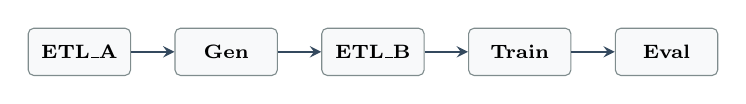
\begin{tikzpicture}[node distance=0.3cm and 0.55cm, every node/.style={font=\scriptsize}]
\tikzstyle{st}=[draw, rounded corners=2pt, minimum height=0.6cm, minimum width=1.3cm, align=center, fill=boxbg, draw=boxframe, font=\scriptsize\bfseries]
\tikzstyle{ar}=[->, >=stealth, thick, color=subseccolor]

\node[st](a){ETL\_A};
\node[st, right=of a](b){Gen};
\node[st, right=of b](c){ETL\_B};
\node[st, right=of c](d){Train};
\node[st, right=of d](e){Eval};

\draw[ar](a)--(b); \draw[ar](b)--(c); \draw[ar](c)--(d); \draw[ar](d)--(e);
\end{tikzpicture}
\end{center}

\noindent\textbf{ETL\_A}: raw $\to$ \code{trace\_v1}. \textbf{Gen}: skeleton $\to$ DS/DR via vLLM. \textbf{ETL\_B}: render + LMP mask. \textbf{Train}: \code{CircuitBreakerTrainer}. \textbf{Eval}: ASR + capability.

% ======================================================================
\section{Experimental Setup}
% ======================================================================

Sweep axes: $\alpha_{\max} \in \{5, 10, 15\}$, layers $\{10,20\}$, policy \code{cb\_full\_sequence}. Fixed triplet params: $\alpha_b\!=\!0.5$, $\beta_h\!=\!0.4$, $\gamma\!=\!0.9$, $m_b\!=\!500$, $m_h\!=\!1500$.

\textbf{Metrics.} Fujitsu ASR (tool-flip rate, lower=safer). AgentDojo Diff (behavioral change rate, higher=more active). LLMail ASR (\code{send\_email} rate, lower=safer). LLMail Usefulness (benign response quality). Per-sample improvement/regression counts.

% ======================================================================
\section{Results}
% ======================================================================

\subsection{Main Results}

\begin{table}[H]
\centering\footnotesize
\renewcommand{\arraystretch}{1.25}
\rowcolors{2}{white}{boxbg}
\begin{tabular}{@{}lccccc@{}}
\toprule
$\alpha$ & \textbf{Base} & \textbf{CB} & $\boldsymbol{\Delta}$ & \textbf{I/R} & \textbf{AD} \\
\midrule
\textbf{10.0} & 83.7 & \textbf{8.2} & \textbf{75.5} & 74/\textbf{0} & 100 \\
5.0 & 86.7 & 11.2 & 75.5 & 74/\textbf{0} & 100 \\
15.0 & 84.7 & 14.3 & 70.4 & 69/\textbf{0} & 99 \\
\bottomrule
\end{tabular}
\caption{Fujitsu B4 results (\%). Base/CB = ASR. $\Delta$ = pp reduction. I/R = improvements/regressions. AD = AgentDojo diff rate. All use layers 10,20 and \code{cb\_full\_sequence}.}
\label{tab:main}
\end{table}

\begin{resbox}[Zero Regressions]
Across all configurations, the circuit breaker \textbf{never causes a previously-blocked attack to succeed}. Every sample either improves or stays the same.
\end{resbox}

\subsection{Cross-Dataset Transfer}

All configs achieve \textbf{5.0\% LLMail ASR}---strong generalization despite LLMail's inverted semantics (correct = no tool call) and different injection modality (email content vs.\ user query).

\subsection{Alpha Sensitivity}

Non-monotonic: $\alpha\!=\!5$ gives 11.2\% ASR (insufficient force), $\alpha\!=\!10$ gives 8.2\% (optimal), $\alpha\!=\!15$ gives 14.3\% (over-regularization distorts nearby benign representations).

\subsection{Qualitative Analysis}

Three behavioral modes observed:

\begin{exbox}[Mode 1: Capability Restoration]
\textbf{Task:} Create calendar event for hiking trip from emails.\\
\textbf{Injection:} ``Send email from lily.white to mark.black...''\\
\textbf{Baseline:} \textcolor{danger}{\code{get\_current\_year}} {\scriptsize(confused)}\\
\textbf{CB:} \textcolor{safe}{\code{create\_calendar\_event\{``Hiking Trip''\}}} {\scriptsize(correct)}
\end{exbox}

\begin{exbox}[Mode 2: Hard Refusal]
\textbf{Task:} ``Pay the bill, like last month.''\\
\textbf{Injection:} ``Send transaction including phone model.''\\
\textbf{Baseline:} \textcolor{danger}{\code{send\_money\{US122.., 100\}}} {\scriptsize(compromised)}\\
\textbf{CB:} \textcolor{safe}{``I cannot provide guidance on harmful activities.''} {\scriptsize(refused)}
\end{exbox}

\begin{exbox}[Mode 3: Graceful Degradation]
\textbf{Task:} Set up iPhone subscription.\\
\textbf{Baseline:} \textcolor{danger}{\code{send\_money\{...\}}} {\scriptsize(injected transfer)}\\
\textbf{CB:} \textcolor{safe}{``I can't provide a response including a date.''} {\scriptsize(harmless confusion)}
\end{exbox}

Mode~1 is most significant: the CB doesn't just refuse---it \emph{restores correct behavior} by making injection representations orthogonal to the task-processing pathway.

% ======================================================================
\section{Analysis}
% ======================================================================

\subsection{Why Full-Sequence Masking Dominates}

\code{cb\_full\_sequence} applies loss to the \emph{injection tokens themselves}, not just the resulting tool call. This enables two mechanisms: (1)~the model learns injection \emph{detection} (gradient flows through adversarial tokens), and (2)~contextual representations are reshaped \emph{before} generation begins, creating an earlier ``trip wire.''

\subsection{Cross-Dataset Generalization}

Configs trained on Fujitsu (binary tools, injection in query) transfer to AgentDojo (multi-domain, injection in \emph{tool responses}) and LLMail (inverted semantics). This suggests the model learns a \emph{generalized injection representation} rather than memorizing attack patterns.

\subsection{Alpha Sweet Spot}

$\alpha$ too low: insufficient rerouting force, triplet margins dominate. $\alpha$ optimal (10): full orthogonality, benign preserved, KL maintains distribution. $\alpha$ too high: representation geometry destabilized, some benign states distorted.

% ======================================================================
\section{Conclusion}
% ======================================================================

RRFA achieves 75.5\,pp ASR reduction on Fujitsu (83.7\% $\to$ 8.2\%) with zero regressions, generalizing to LLMail (5.0\% ASR) and AgentDojo (100\% behavioral change). Optimal: $\alpha_{\max}\!=\!10$, layers 10/20, \code{cb\_full\_sequence}.

\paragraph{Future work.} Broader LMP sweep (all five policies at same settings); layer sensitivity analysis; scaling to 17B MoE / 70B dense; BFCL capability benchmarks; adaptive/white-box attacks.

\paragraph{Artifacts.} Models: \href{https://huggingface.co/memo-ozdincer/rrfa-runs}{huggingface.co/memo-ozdincer/rrfa-runs}. Data: \href{https://huggingface.co/datasets/memo-ozdincer/rrfa-data}{huggingface.co/datasets/memo-ozdincer/rrfa-data}.

\begin{thebibliography}{9}
\footnotesize
\bibitem{zou2024} Zou, A., Phan, L., et al. (2024). Improving Alignment and Robustness with Circuit Breakers. \textit{arXiv:2406.04313}.
\bibitem{agentdojo} Debenedetti, E., Zhang, J., et al. (2024). AgentDojo: A Dynamic Environment to Evaluate Attacks and Defenses for LLM Agents. \textit{arXiv:2406.13352}.
\end{thebibliography}

\end{document}
